\section{Actividad 7}

\subsection*{Diseñar en GNU Radio un modulador que genere una señal de Doble Banda Lateral con Portadora Suprimida. Indicar cuál es la diferencia de espectro con la señal del ejercicio anterior.}

Se diseña un modulador que permite generar una señal de Doble Banda Lateral con
Portadora Suprimida, el mismo se muestra en la Fig. \ref{fig:diseño_7}. Para generar una señal DSB-SC, sólo es necesario un bloque que multiplique la portadora con la señal del mensaje.

    \begin{figure}[H]
        \centering
        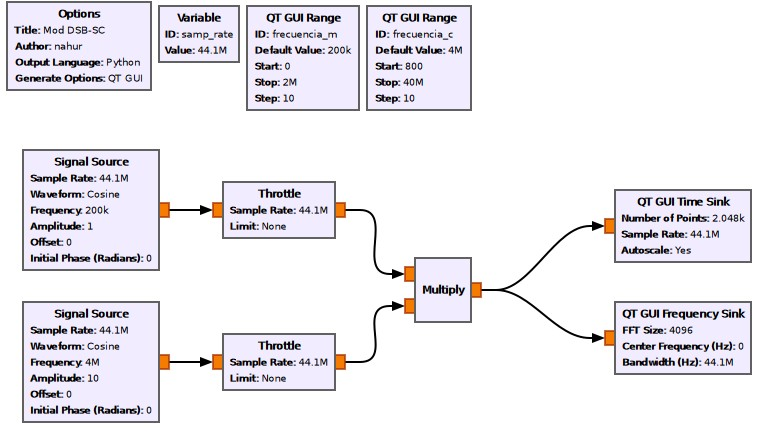
\includegraphics[width=0.7\linewidth]{imagenes/Parte_1/Actividad_7/ejercicio_7.jpg}
        \caption{Diseño de una BLS-SC.}
        \label{fig:diseño_7}
    \end{figure}

En la Fig. \ref{fig:espectro_7} se puede apreciar la señal $s (t)$ en el dominio del tiempo así como su espectro en el dominio de la frecuencia, además también se aprecia que la señal portadora ya no aparece y esto se debe al tipo de modulación que se está diseñando para suprimir dicha portadora.

    \begin{figure}[H]
        \centering
        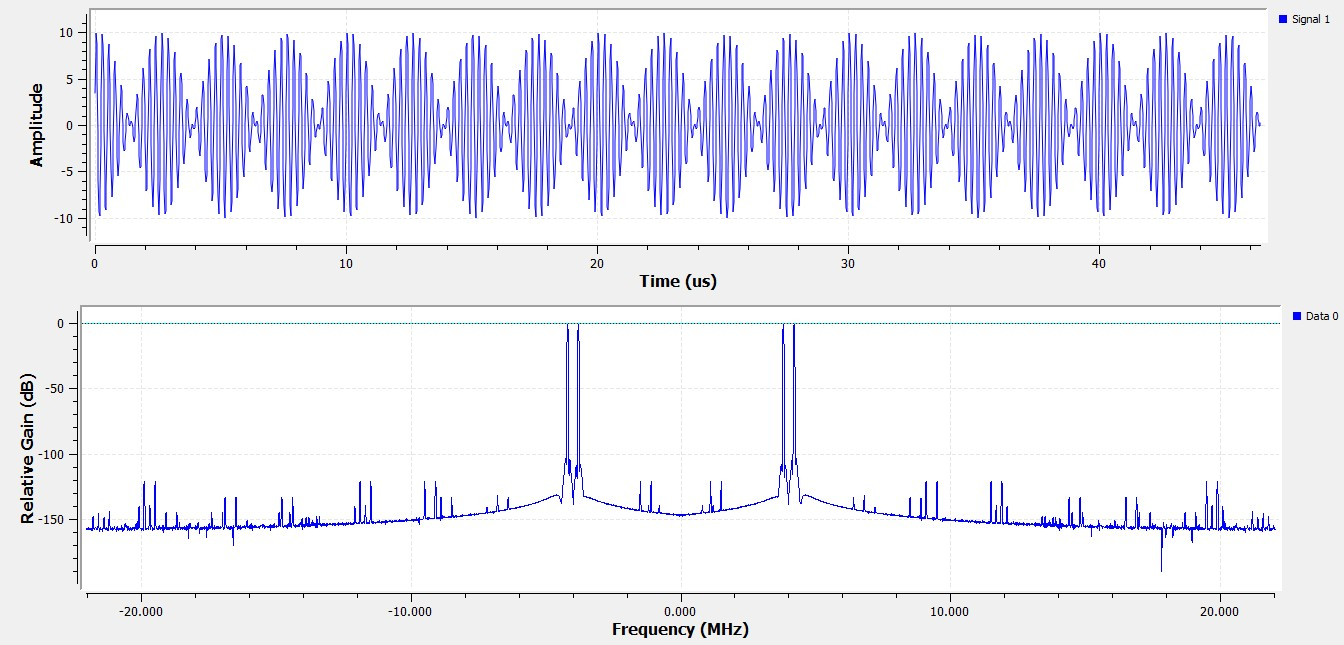
\includegraphics[width=0.9\linewidth]{imagenes/Parte_1/Actividad_7/ejercicio_7_espectro.jpg}
        \caption{Señal s(t).}
        \label{fig:espectro_7}
    \end{figure}
    